\documentclass{newsiambook}
%\newcommand{\ProgrammingLanguage}{matlab}
\newcommand{\ProgrammingLanguage}{python}

\usepackage{hyperref}
\usepackage{import}
\usepackage{amsmath, amsfonts, amscd, amssymb}
\usepackage{mathtools}
\usepackage{epsfig}
\usepackage{graphicx}
\usepackage{url}
\usepackage{mathrsfs}
\usepackage{makeidx}
\usepackage{multicol}
\usepackage{color}
\usepackage{crop}
%\usepackage{appendix}
\usepackage{verbatim}
\usepackage{listings}
\usepackage{pseudocode}
\usepackage{framed}
%\usepackage{caption}
%\usepackage{fontspec}
%\usepackage[T1]{fontenc}
%\usepackage{beramono}
%\usepackage{caption}
%\DeclareCaptionFont{white}{\color{white}}
%\DeclareCaptionFormat{listing}{\colorbox[cmyk]{0.43, 0.35, 0.35,0.01}{\parbox{\textwidth}{\hspace{15pt}#1#2#3}}}
%\captionsetup[lstlisting]{format=listing,labelfont=white,textfont=white, singlelinecheck=false, margin=0pt, font={bf,footnotesize}}

%\usepackage{sagetex}
\usepackage{versions}
\usepackage{ifthen}
\newenvironment{amatrix}[1]{%
\left(\begin{array}{@{}*{#1}{c}|c@{}}
}{%
\end{array}\right)
}

\newenvironment{dmatrix}[2]{%
\left(\begin{array}{@{}*{#1}{c}|*{#2}{c}@{}}
}{%
\end{array}\right)
}

\newenvironment{pseudo}[2]
    {\begin{pseudocode}[shadowbox]{#1}{#2}}
    {\end{pseudocode}}

\newenvironment{problem}{\begin{shaded}\begin{problemnum}}{\end{problemnum}\end{shaded}}

\newtheoremup{problemnum}{Problem}
\definecolor{shadecolor}{gray}{0.90}

\newcommand{\li}[1]{\lstinline[style=python]!#1!}

\newcommand{\ipt}[2]{\langle #1,#2 \rangle}
\newcommand{\ip}{\int_{-\infty}^{+\infty}}

\renewcommand{\ker}[1]{\mathcal{N}(#1)}
\newcommand{\ran}[1]{\mathcal{R}(#1)}

\makeatletter
\g@addto@macro\@floatboxreset\centering
\makeatother

\DeclareMathOperator{\res}{res}           % Residue
\DeclareMathOperator{\Res}{Res}           % Residue


\def\0{{\bf 0}}
\def\a{{\bf a}}
\def\b{{\bf b}}
\def\e{{\bf e}}
\def\p{{\bf p}}
\def\q{{\bf q}}
\def\u{{\bf u}}
\def\v{{\bf v}}
\def\w{{\bf w}}
\def\x{{\bf x}}
\def\y{{\bf y}}
\def\z{{\bf z}}
\def\subspace{\lhd}

\def\CalL{\mathcal{L}}
\def\CalO{\mathcal{O}}
\def\CalV{\mathcal{V}}
\def\CalU{\mathcal{U}}
\def\bU{{\bar{u}}}
\def\R{\Re e}
\def\I{\Im m}
\def\M{M_n}

\lstset{basicstyle=\footnotesize\ttfamily,
        keywordstyle=\color{blue}\bfseries,
        tabsize=4,
        frame=tb,
        captionpos=b,
        title=\lstname,
        abovecaptionskip=-5pt,
        belowcaptionskip=-5pt,
        breaklines=true,
        breakatwhitespace=false,
        showstringspaces=false}

\lstdefinestyle{fromfile}{frame=single
                          numbers=left,
                          numberstyle=\tiny,
                          stepnumber=2,
                          numbersep=7pt,
                          numberfirstline=true,
                          abovecaptionskip=10pt,
                          belowcaptionskip=10pt}

\lstset{basicstyle=\footnotesize\ttfamily,
		keywordstyle=\color{blue}\bfseries\ttfamily,
		tabsize=4,
		frame=tb,
		captionpos=b,
		breaklines=true,
		breakatwhitespace=false,
		title=\lstname,
		showstringspaces=false}



%----PYTHON STYLES----                          
\lstdefinestyle{python}{language=Python}
\lstdefinestyle{pythonnums}{language=Python,
                            numbers=left,
                            numberstyle=\tiny,
                            stepnumber=2,
                            numbersep=7pt,
                            numberfirstline=true}
\crop
\makeindex
\newcommand{\objective}[1]{\vspace{5mm}{\bf Lesson Objective: } \emph{#1} \setcounter{problemnum}{0} \setcounter{equation}{0} \vspace{5mm}}
\renewcommand{\chaptername}{Lab}

\newcommand{\lab}[3]{\chapter[#3]{#1: #2}}
\providecommand{\abs}[1]{\lvert#1\rvert}
\providecommand{\norm}[1]{\lVert#1\rVert}


%\newcommand{\PythonVersion}{1}

% \captionsetup{style=base,
%               labelformat=default,
%               labelsep=endash,
%               justification=raggedright}

%\includeonly{./Applications_Combined/PageRank}
%\includeonly{./Algorithms_PyLabs/Complexity_py}
\begin{document}

%-------------------------------------------------------------
%This section is logic that switches from one language to another. Maybe it should be in another file...
\ifthenelse{\equal{\ProgrammingLanguage}{python}}
{
  \includeversion{python}
  \excludeversion{matlab}
  \newcommand{\li}[1]{\lstinline[style=python]!#1!}
  %\renewcommand{\lstincludelisting}[2]{\lstincludelisting[style=python]{#2}}
  \renewcommand{\ProgrammingLanguage}{Python }

  %table of commands
  %\newcommand{\inverse}{la.inv()}
}{}

\ifthenelse{\equal{\ProgrammingLanguage}{matlab}}
{
  \includeversion{matlab}
  \excludeversion{python}
  \newcommand{\li}[1]{\lstinline[style=matlab]!#1!}
  %\renewcommand{\lstincludelisting}[2]{\lstincludelisting[style=matlab]{#2}}
  \renewcommand{\ProgrammingLanguage}{MATLAB }

  %table of commands
  %\newcommand{\inverse}{inv}
}{}

\lstset{basicstyle=\footnotesize\ttfamily,
        keywordstyle=\color{blue}\bfseries,
        tabsize=4,
        frame=tb,
        captionpos=b,
        title=\lstname,
        abovecaptionskip=-5pt,
        belowcaptionskip=-5pt,
        breaklines=true,
        breakatwhitespace=false,
        showstringspaces=false}

\lstdefinestyle{fromfile}{frame=single
                          numbers=left,
                          numberstyle=\tiny,
                          stepnumber=2,
                          numbersep=7pt,
                          numberfirstline=true,
                          abovecaptionskip=10pt,
                          belowcaptionskip=10pt}

%----PYTHON STYLES----                          
\lstdefinestyle{python}{language=Python}
\lstdefinestyle{pythonnums}{language=Python,
                            numbers=left,
                            numberstyle=\tiny,
                            stepnumber=2,
                            numbersep=7pt,
                            numberfirstline=true}

%----MATLAB STYLES----
\lstdefinestyle{matlab}{language=Matlab}
\lstdefinestyle{matlabnums}{language=Matlab,
                            numbers=left,
                            numberstyle=\tiny,
                            stepnumber=2,
                            numbersep=7pt,
                            numberfirstline=true}

\newenvironment{pseudo}[2]
    {\begin{pseudocode}[shadowbox]{#1}{#2}}
    {\end{pseudocode}}

%----------------------------------------------------------------
%Book cover and Front matter
\thispagestyle{empty}
\begin{center}
{\Huge \bf Applied Mathematics and Computing}

\vspace{10mm}
{\Large \bf \ProgrammingLanguage Edition}

\vspace{20mm}

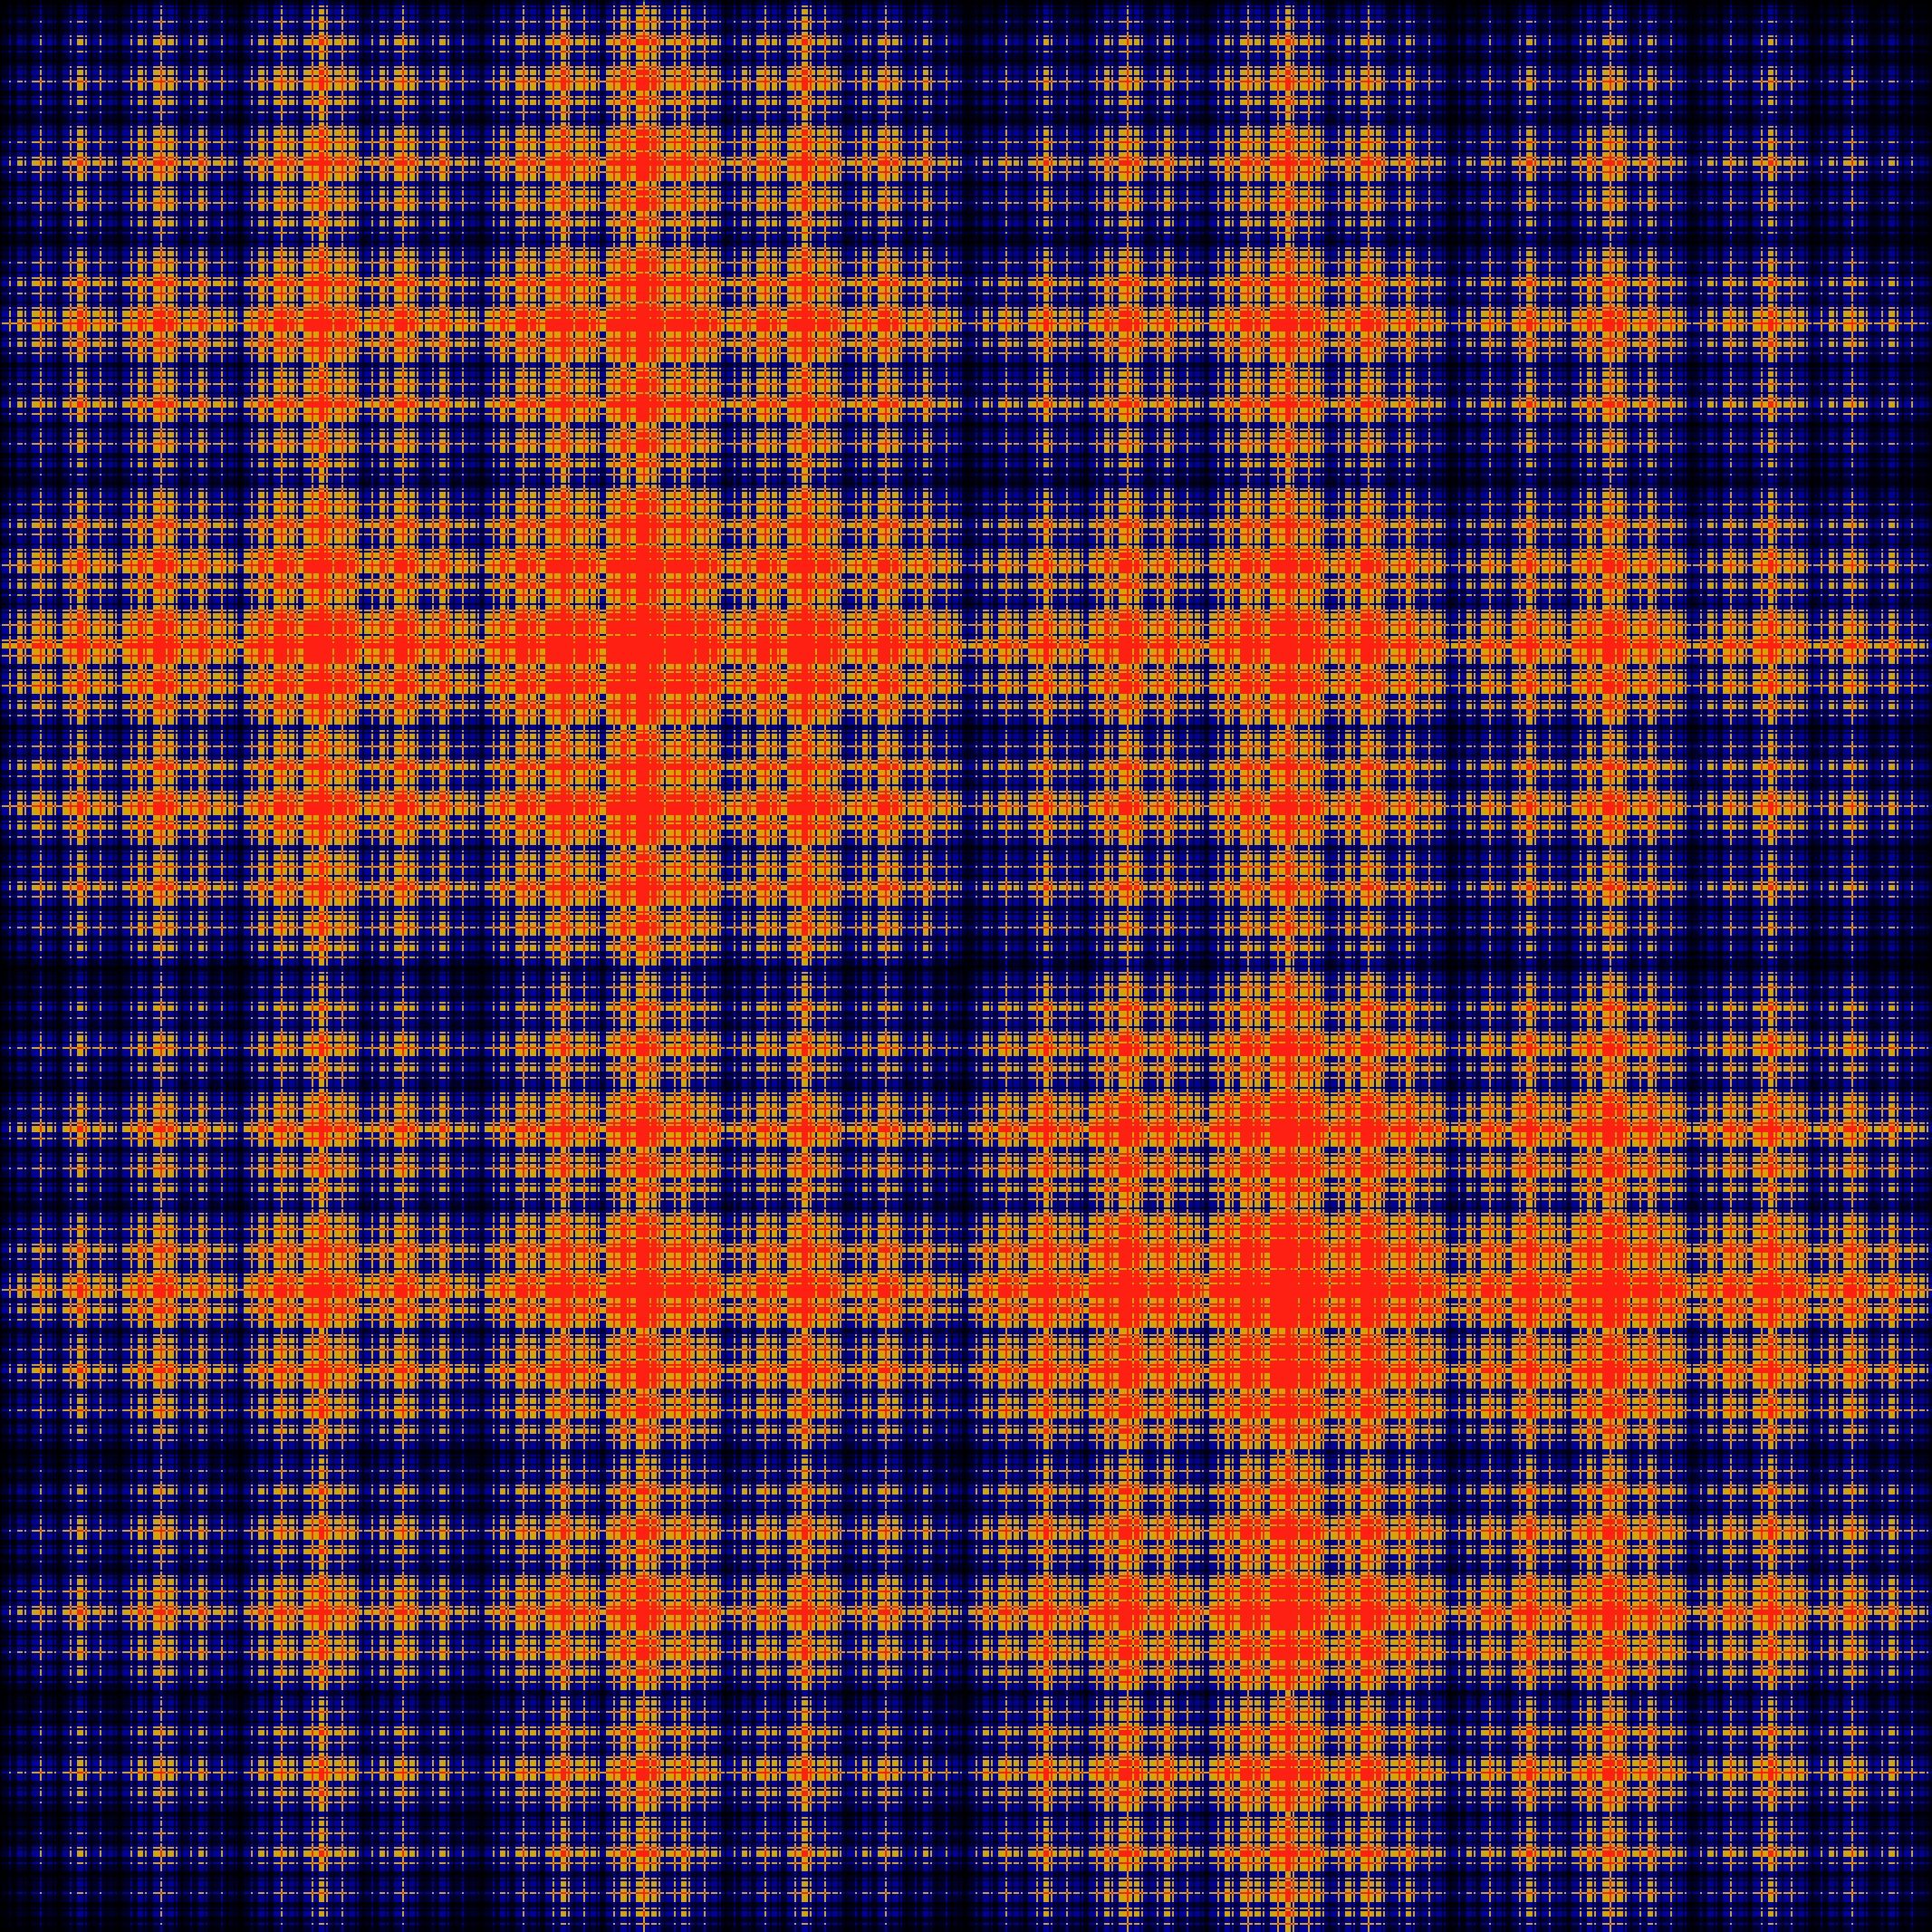
\includegraphics[scale = .25]{Cover}
\end{center}
\frontmatter
\begin{contributors}
\contributor{J.~Humpherys}{Brigham Young University}
\contributor{J.~Webb}{Brigham Young University}
\contributor{R.~Murray}{Brigham Young University}
\contributor{J.~West}{University of Michigan}
\contributor{R.~Grout}{Brigham Young University}
\contributor{K.~Finlinson}{Brigham Young University}
\end{contributors}

%------------------------------------------------------------------
%The preface, which will presumably be longer in the future

\begin{thepreface}
This lab manual is designed to accompany the textbook \emph{Foundations of Applied Mathematics} by Dr.~J.~Humpherys.

\vfill
\copyright{This work is licensed under the Creative Commons Attribution 3.0 United States 
License.  You may copy, distribute, and display this copyrighted work only if you give 
credit to Dr.~J.~Humpherys. All derivative works must include an attribution to Dr.~J.~Humpherys as the owner of this work as well as the web address to 
\\\centerline{\url{https://github.com/ayr0/numerical_computing}}\\ as the original source of 
this 
work.\\To view a copy of the Creative Commons Attribution 3.0 License, 
visit\\\centerline{\url{http://creativecommons.org/licenses/by/3.0/us/}} or send a letter to 
Creative Commons, 171 Second Street, Suite 300, San Francisco, California, 94105, USA.}

\vfill
\centering
\includegraphics[height=1.2cm]{by}
\vfill
\end{thepreface}
%-----------------------------------------------------------------

\setcounter{tocdepth}{1}
\tableofcontents

\mainmatter

%-----------------------------------------------------------------
%Programming Tutorials are in the following sections. They are split into different files dependent upon language

\begin{python}
%Python programming tutorials
\subimport{Ch0_Py/}{Py0}

\subimport{./Algorithms/Matrices/}{Matrices1}
\subimport{./Algorithms/Matrices/}{Matrices2}

\subimport{./Algorithms/Functions/}{Functions}
\end{python}

\begin{matlab}
%Matlab programming tutorials
\subimport{./Ch0_MAT/}{Ch0V2}

\subimport{./Algorithms/MatricesM/}{Matrices1}
\subimport{./Algorithms/MatricesM/}{Matrices2}

\subimport{./Algorithms/FunctionsM/}{Functions}
\end{matlab}

\subimport{./Applications/MarkovGraph/}{MarkovGraph_C}




%----------------------------------------------------------
%The Elementary Matrices lab is combined into one file

\subimport{./Algorithms/ElemMatrices/}{ElemMatr_C}

%-----------------------------------------------------------
%The next few labs are more programming tutorial labs, and are split by language
\begin{python}
\subimport{./Algorithms/Conditionals/}{Conditionals}
\subimport{./Algorithms/Complexity/}{Complexity}
\end{python}

\begin{matlab}
\subimport{./Algorithms/ConditionalsM/}{Conditionals}
\subimport{./Algorithms/ComplexityM/}{Complexity}
\end{matlab}

\subimport{./Applications/Leontief/}{Leontief_C}

%-----------------------------------------------------------
%These labs are primarily Linear Algebra Labs (Factorizations and Applications)
%They are combined

\subimport{./Algorithms/QR/}{QR_C}
\subimport{./Applications/Statistics/}{Stats1_C}
\subimport{./Algorithms/CanonTransform/}{CanonTransform} 
\subimport{./Applications/OrthoPoly/}{OrthoPoly_C}

\subimport{./Algorithms/EigSolver/}{Eig_C}
\subimport{./Applications/EigGraph/}{EigGraph_C}

\subimport{./Algorithms/Cholesky/}{Cholesky_C}
\subimport{./Applications/SVD/}{SVD_C}

%------------------------------------------------------------
%These labs are more advanced programming labs. They are separated by language.

\begin{python}
\subimport{./Algorithms/Functions/}{Functions2}
%\subimport{./Applications/Vectorization/}{Vectorization}

\subimport{./Applications/Recursion/}{Recursion}
%We need a profiler lab here.

\end{python}

\begin{matlab}
\subimport{./Algorithms/FunctionsM/}{Functions2}
\subimport{./Applications/Vectorization}{Vectorization}

\subimport{./Applications/RecursionM}{Recursion}
%\subimport{./Algorithms_MATLabs}{Profiler}
\end{matlab}

\subimport{./Applications/NormsGeometry/}{Norms_Geometry}

%-----------------------------------------------------------
%These labs cover the basics of differentiation, Newton's method and a number of related applications. These are combined labs

\subimport{./Algorithms/NumDeriv/}{FiniteDiff_C}
\subimport{./Applications/BeamBuckle/}{Beams_C}

\subimport{./Algorithms/MultiDeriv/}{FiniteDiff2_C}
\subimport{./Applications/ImgFilters/}{ImgFilters}

\subimport{./Applications/NewtonsMethod/}{Newton_C}
\subimport{./Applications/LevelSet/}{LevelSet}

\subimport{./Algorithms/Broyden/}{Broyden}
\subimport{./Applications/Julia/}{Julia}

\subimport{./Applications/PageRank/}{PageRank}
\subimport{./Algorithms/JacobiGaussSidel/}{Iterative1}
\subimport{./Algorithms/SuccOverRelax/}{Iterative2}
%Need permission and web address for internet.dat

%==================================================
%End of the first half
%==================================================


%---------------------------------------------------------------
%These labs cover integration and approximation theory. They are combined labs


%These labs still need to be merged/translated

\subimport{./Algorithms/Barycentric/}{Barycentric}
\subimport{./Applications/MC/}{MC}

\subimport{./Algorithms/NewtonCotes/}{NCInteg}
\subimport{./Applications/VarianceReduction/}{VEGAS}

\subimport{./Algorithms/Splines/}{Splines}
\subimport{./Applications/Tesselation/}{Tess}

\subimport{./Algorithms/GaussQuad/}{GaussQuad}
\subimport{./Applications/NURBS/}{NURBS_C}

%---------------------------------------------------------------
%This is one lab about more advanced visualization topics. It will be split by language

\begin{matlab}
\subimport{./Algorithms/SciVizM/}{SciViz}
\end{matlab}

\begin{python}
\subimport{./Algorithms/SciViz/}{SciViz}
\end{python}

%---------------------------------------------------------------
%A few labs related to complex mappings and the perspective transform. These labs are combined.

%These labs need translation and merging

\subimport{./Applications/ConfMaps/}{ConfMaps}

\subimport{./Algorithms/PerspectiveTransform/}{PerspTrans_C}
\subimport{./Applications/RiemannSphere/}{RiemannSphere_C}

%---------------------------------------------------------------
%These labs cover plotting and visualization. They will be separated by language

\begin{matlab}
%\subimport{./Algorithms/}{GraphicsHandles}
%\subimport{./Applications_MATLabs/}{TimeDelay}

%\subimport{./Algorithms_MATLabs/}{Motion3D}
\end{matlab}

\begin{python} 
%\subimport{./Algorithms_PyLabs/}{GraphicsHandles}
%\subimport{./Applications_PyLabs/}{TimeDelay}

%\subimport{./Algorithms_PyLabs/}{Motion3D}
\end{python}

%----------------------------------------------------------------
%These labs cover a wide variety of applications, and finish off the book. They will be combined

%\subimport{./Applications/RayTracing/}{RayTracing}

\subimport{./Algorithms/JordanSchur/}{Jordan}
\subimport{./Applications/LagSylvInterp/}{LagSylvInterp}

\subimport{./Algorithms/Krylov/}{Krylov}
\subimport{./Applications/MarkovPerron/}{MarkovPerron}

\subimport{./Algorithms/MoorePenrose/}{MP}
\subimport{./Applications/MoorePenrose/}{MPApp}
%\lab{Algorithms}{Moore-Penrose Pseudo-Inverse}{Moore-Penrose}

\objective{This section explains several methods for numerically computing the Moore-Penrose Pseudo-Inverse. It also compares performance of the different methods.}
 
The generalized inverse of a matrix $A$ is a matrix (which we will denote $A^\dagger$ for now) that satisfies the following:
\begin{equation} \label{cond:one}
AA^\dagger A = A 
\end{equation}

\begin{equation} \label{cond:two}
A^\dagger A A^\dagger = A^\dagger 
\end{equation}

For any matrix $A$ there exists a generalized inverse. Note that in the case that $A$ is invertible, $A^{-1}$ satisfies the conditions \ref{cond:one} and \ref{cond:two}. However, it is not generally unique. For this reason, we usually add additional conditions that make the generalized inverse unique.

For example, we can specify the following two additional conditions:

\begin{equation} \label{cond:three}
(AA^\dagger)^* = AA^\dagger
\end{equation}

\begin{equation} \label{cond:four}
(A^\dagger A)^* = A^\dagger A
\end{equation}

These four conditions guarantee both the existence and uniqueness of the matrix $A^\dagger$ for any matrix $A$. The matrix $A^\dagger$ is known as the Moore-Penrose inverse. In some settings it is simply called the pseudo-inverse.\footnote{For the rest of this section we will use the notation $A^\dagger$ to represent the moore-penrose inverse, although in some books that notation is used a generalized inverse}

{\bf We could add some exposition here about examples of the MP inverse for specific matrices, but I don't know if Jeff is doing that in the book or not...}

\subsection{Calculating the Moore-Penrose Inverse}

There are several different methods for calculating the Moore-Penrose Inverse. We will consider the most general method first, and then compare its performance to a few specialized methods.

Recall that the SVD of a matrix $A$ is of the form

\[
A = U \Sigma V^*
\]

Where $U$ and $V$ are unitary (i.e. $U^*U = I$) and $\Sigma$ is diagonal. Consider the matrix

\[
B = V \Sigma^\dagger U^*
\]

Where $\Sigma^\dagger$ is the pseudo-inverse of $\Sigma$. Since $\Sigma$ is diagonal, the pseudo-inverse is simply found by replacing each non-zero entry with its multiplicative inverse and transposing the matrix. We write, for ease of notation $\Sigma^\dagger \Sigma = I_A$ Now we have the following:

\[
ABA = U \Sigma V^* = A
\]

\[
BAB = V \Sigma^\dagger U^* = B
\]

\[
(AB)^* = U \Sigma^{\dagger *} V^* V \Sigma^* U^* = U (\Sigma \Sigma^\dagger)^* U^* = U \Sigma \Sigma^\dagger U^* = U \Sigma V^* V \Sigma^\dagger U^* = AB
\]

\[
(BA)^* =  V \Sigma^* U^* U \Sigma^{\dagger *} V^* = V (\Sigma^\dagger \Sigma)^* V^* = V  \Sigma^\dagger \Sigma V^* =  V \Sigma^\dagger U^* U \Sigma V^* = BA
\]

Thus $B$ satisfies all of the properties of the pseudo-inverse, and since the pseudo-inverse is unique it is the only such matrix.

Therefore, we can easily calculate the pseudo-inverse of a matrix using the SVD. Write the following code in \ProgrammingLanguage :

\begin{matlab}
\begin{lstlisting}[style=matlab]
[U,S,V] = svd(A,'econ');
\end{lstlisting}
\end{matlab}
\begin{python}
\begin{lstlisting}[style=python]
U,s,Vh = la.svd(A,full_matrices=False)
S = sp.diag(s)
\end{lstlisting}
\end{python}

\begin{matlab}%I don't know if the following is true of the Python version yet
As you recall, in chapter three we talked about how the \li{econ} option for the \li{svd} function makes the SVD representation as compact as possible, by eliminating the sections of $\Sigma$ that are zeros, and the corresponding parts of $U$ and $V$. \end{matlab}We can then calculate the pseudo-inverse by using the following line of code:

\begin{matlab}
\begin{lstlisting}[style=matlab]
Apinv = V*diag(1./diag(S))*U';
\end{lstlisting}
\end{matlab}
\begin{python}
\begin{lstlisting}[style=python]
Apinv = sp.dot(sp.dot(Vh.T,sp.diag(1./s)),U.T)
\end{lstlisting}
\end{python}

This line uses the matrices that \li{svd} created to calculate the pseudo-inverse, using the formula we established above. Note that we used \li{diag} twice to invert just the singular values (and not the zeros). \begin{matlab}Also note that since we used the \li{econ} option the matrix $S$ is square and hermitian, and therefore we don't have to transpose it.\end{matlab}%still don't know if this is valid for the full_matrices=0 option
\begin{problem}
\begin{matlab}
\ProgrammingLanguage has a built-in function \li{pinv}that calculates the pseudo-inverse. Write a script that compares the performance of \li{pinv} and the implementation that we demonstrated above. Use a matrix generated by  \li{rand}.\end{matlab}
\begin{python}%Python has pinv and pinv2, which appear to differ by algorithms. So which one do we test? - I think pinv2 uses SVD -- here I suggest to test both
\ProgrammingLanguage has the built-in functions \li{la.pinv} and \li{la.pinv2} to calculate the pseudo-inverse. Write a script that compares the performance of \li{la.pinv},\li{la.pinv2}, and the implementation that we demonstrated above. Use a matrix generated by  \li{sp.rand}.\end{python}
 Try the following matrix sizes:
\begin{itemize}
\item $1000 \times 1$
\item $1000 \times 20$
\item $1000 \times 500$
\item $1000 \times 1000$
\end{itemize}
How do the performances compare?
\end{problem}

\begin{problem}
{\bf Continuity of the pseudo-inverse:} This problem demonstrates why the pseudo-inverse is not generally a continous operation. Create a random $5 \times 5$ matrix $A$, and find its SVD using the code:
%should we use 'econ' here? I haven't read whatever section that comes from
\begin{matlab}
\begin{lstlisting}[style=matlab]
[U,S,V] = svd(A)
\end{lstlisting}
\end{matlab}
\begin{python}
\begin{lstlisting}[style=python]
U,s,Vh = la.svd(A,full_matrices=False)
V = Vh.T
S = sp.diag(s)
\end{lstlisting}
\end{python}.
Set the bottom right entry of $S$ to zero, and then set $A = U*S*V'$. Now set $S(5,5)$ to be $.01$. Now calculate \begin{matlab}\li{norm(A - U*S*V')}\end{matlab}\begin{python}\li{la.norm(A - sp.dot(sp.dot(U,S),Vh))}\end{python}. The value should be $.01$. This is because the matrix $2$-norm is simply the value of the largest singular value. Now calculate \begin{matlab}\li{norm(pinv(A) - pinv(U*S*V'))}\end{matlab}\begin{python}\li{la.norm(la.pinv(A) - la.pinv(sp.dot(sp.dot(U,S),Vh)))}\end{python}. You should get $100$. Why is this? Hint: Think of how we calculated the pseudo-inverse. This example, and your explanation, should explain why two matrices, that are arbitrarily close together, can have pseudo-inverses that are arbitrarily far apart. Thus the pseudo-inverse is not a continuous operator.
\end{problem}

\subsection*{Other methods for calculating the Pseudo-Inverse}

The SVD is a powerful tool for calculating the pseudo-inverse. However, for large matrices it can be costly to calculate the SVD. Accordingly, there are several other methods for calculating the pseudo-inverse of a matrix.

One method is an iterative approach established by Ben-Israel and Cohen\footnote{Ben-Israel, Adi; Cohen, Dan (1966). "On Iterative Computation of Generalized Inverses and Associated Projections". SIAM Journal on Numerical Analysis 3: 410–419.}. This method uses the recursive sequence

\[
A_{i+1} = 2A_i - A_i A A_i
\]

With $A_0$ satisfying the equation $A_0 A = (A_0 A)^*$. The convergence of this sequence eventually becomes quadractic, which is a very desirable property. The simplest choice for $A_0$ is $\alpha A^*$, with $0 < \alpha < 2/\sigma_1^2(A)$, where $\sigma_1$ denotes the largest singular value (the condition on $\alpha$ is a technical condition established in the original paper to guarantee fast convergence).

One tricky part of developing this method is finding an appropriate $\alpha$. We don't want to waste much time calculating $\sigma_1$. Luckily there is an easy equivalence that we can leverage:

\[
||A||_2 = \sigma_1(A) = \sqrt{\lambda_{max} (A^* A)}
\]
%Python: no eigs function -- but it appears to be a topic of interest in the community, perhaps a future addition
Thus, we can calculate the largest singular value of $A$ quickly in some cases using \begin{matlab}\li{eigs}\end{matlab}. We stress that this is not always the fastest way. For example, if $A$ is a million by one column vector then calculating the 2-norm of $A$ is much faster than calculating the largest eigenvalue of a million by million matrix. However, with these equivalences we have some tools at our disposal to easily calculate the largest singular value of $A$.

Now, using these tools, we can write a simple function to calculate the pseudo-inverse using this iterative method:

\begin{matlab}
\begin{lstlisting}[style=matlab]
function out = IterativePInv(A)

alpha = 2/(1.1*eigs(A'*A,1));
out = alpha*A';
C = out + 1;
while max(sum(abs(C-out))) > 1e-4
    C = out;
    out = 2*out - out*A*out;
end
\end{lstlisting}
\end{matlab}
\begin{python}
\begin{lstlisting}[style=python]
function out = IterativePInv(A)

alpha = 2/(1.1*eigs(A'*A,1));
out = alpha*A';
C = out + 1;
while max(sum(abs(C-out))) > 1e-4
    C = out;
    out = 2*out - out*A*out;
end
\end{lstlisting}
\end{python}
As you can see, the implementation of this algorithm is fairly straightforward. We used the matrix $1$-norm (the maximum absolute column sum) to detect convergence of our sequence, since it is very fast to compute.

\begin{problem}
The implementation we wrote above is naive in a few ways. Make the following three adaptations to your code:
\begin{itemize}
\item Allow variable tolerance in the detection of convergence of the sequence. Use \begin{matlab}\li{varargin}\end{matlab}\begin{python}\li{*args}\end{python} so that the user only specifies the tolerance if they want to.
\item We used the value $1.1$ rather arbitrarily in our selection of $\alpha$. The original paper proves that the optimal value is $2/(\sigma_1^2 + \sigma_r^2)$, where $\sigma_r$ is the smallest non-zero singular value. Use \begin{matlab}\li{eigs}\end{matlab} again to find the value of $\sigma_r$, and use that value to set $\alpha$.
\item If $A$ isn't close to square then it is not advantageous to use \begin{matlab}\li{eigs}\end{matlab} at all, as we explained above. Adapt the code to only use \li{eigs} as you think it's appropriate. Remember that you can use the matrix $2$-norm and a constant like $1.1$ in cases where \begin{matlab}\li{eigs}\end{matlab} isn't appropriate.
\end{itemize}

Now test your code against the svd method, using the same cases that you did for that method. How does it perform?
\end{problem}

It should be noted that this method, although powerful, sometimes performs worse than the svd method. Specifically, when the matrix is ill-conditioned, it may take a long time for the sequence to enter the region of quadratic convergence, making this method a poor choice.

\subsection*{The QR method}

This final method, while only applicable in certain cases, offers a very fast method for calculating the pseudo-inverse. Suppose that $A$ has full column rank. We could show that the pseudo-inverse is then:
\[
A^\dagger = (A^* A)^{-1} A^*
\]

Direct calculation of the pseudo-inverse using this formula is not very helpful, since matrix inversion is so costly. However, since $A$ is full rank, then $A^*A$ is positive definite, and thus has a cholesky decomposition. Therefore, we can rewrite this equation as:

\[
R^*R A^\dagger = A^*
\]

with $R$ being upper-triangular. This equation can be solved quickly by using forward and backward substitution.

We can speed calculation even further by noting that we don't even have to calculate $A^* A$, which can be costly (again, imagine the million by one vector). We can calculate R using the QR-decomposition of A:

\[
A^* A = R^*Q^*QR = R^* R
\]

These equalities hold since $Q$ is orthogonal. Further, in the QR decomposition $R$ is upper-triangular, and thus we can calculate the cholesky factorization easily using the QR decomposition.

Combining these facts we can write the following code to calculate the pseudo-inverse for a matrix that has full column rank as follows:

\begin{matlab}
\begin{lstlisting}[style=matlab]
R = triu(qr(A));

Ainv = R\(R'\A');
\end{lstlisting}
\end{matlab}
\begin{matlab}
\begin{lstlisting}[style=matlab]
R = la.qr(A)[1];

Ainv = la.lstsq(R,la.lstsq(R.T,A.T)[0])[0];
\end{lstlisting}
\end{matlab}

\begin{matlab}We have to use \li{triu} in the first line because of the conventions used by MATLAB's \li{qr} code.\end{matlab}\begin{python}The first line performs QR decomposition for $R$.\end{python} The second line conducts the backwards and forwards substitutions.

\begin{problem}
%This Problem did not exactly work in Python, my function was slower when A was square when using la.lstsq
Compare the run-time of this code against \ProgrammingLanguage's \begin{matlab}\li{pinv}\end{matlab}\begin{python}\li{la.pinv}\end{python}, for the values used in the other problems. \begin{python}Also, make sure to use a non-square matrix for A, or for square matricies change the \li{la.lstsq}'s to \li{la.solve}'s to maximize performance.\end{python}How does it compare? It should be a lot faster. This demonstrates that by leveraging the correct information (full column rank) we can significantly improve the speed of this operation. Note that we can beat \ProgrammingLanguage's own implementation significantly in this case.

\end{problem}

\begin{problem}
This method can also be adapted to use for matrices that have full row rank. In the case of full column rank the following formula holds:
\[
A^\dagger = A^*(A A^*)^{-1}
\]
Use the same technique to write a function that finds the pseudo-inverse for a matrix of full row rank. Note that you will have to find the QR-decomposition of $A^*$ this time, and that it may be helpful to take the transpose so that you can use the backslash operator.
\end{problem}
%Needs to be translated (FWG) --Python Lacks an eigs command, which makes translation of the middle subsection difficult

\subimport{./Algorithms/Drazin/}{Drazin}
\subimport{./Applications/MarkovCount/}{MarkovCount}

%There will be four group theory labs here as well, but we don't have stubs for those yet.

%\appendix
%\appendixpage
%\addappheadtotoc
%\include{simulink}
\end{document}
